\chapter {Projekt}
Głównym celem projektu jest stworzenie i weryfikacja modelu rozprzestrzeniania się ognia wykorzystując niehomogeniczne automaty
komórkowe. Nacisk z pracy został położony na opracowanie algorytmu najdokładniej oddającego rzeczywistość.
Aplikacja, nazwa Sparkle została zaprojektowana tak, aby zapewnić użytkownikowi wysoką ergonomię pracy i łatwość nauki.
Podczas projektowania i implementacji szczególna uwaga została poświęcona dalszym możliwościom rozbudowy programu.
\label{cha:projekt}
\section {Główne zależenia}
\begin {itemize}
\item Projekt obejmuje zarówno stworzenie modelu rozprzestrzeniania pożaru jak i  uproszczonej wizualizacji oraz graficznego interfejsu użytkownika (GUI).
\item Interfejs aplikacji powinien umożliwiać edycję budynku w którym przeprowadzana jest symulacja: dodawanie elementów konstrukcji, 
określanie materiałów z których zostały stworzone. 
\item Użytkownik powinien mieć możliwość określenia źródła ognia: zarówno jego miejsca jak i temperatury początkowej.
\item Aplikacja powinna umożliwiać także kontrolę nad symulacją: możliwość zatrzymania symulacji, wznowienia, rozpoczęcia od początku,
a także dostosowanie tempa symulacji umożliwiającego obserwację zjawisk fizycznych.
\item Dodatkowym elementem jest zapis wyników w postaci rozkładu temperatur do pliku, umożliwiający dogłębną analizę rezultatów.
\item Wizualizacja powinna obejmować zarówno rozkład temperaturowy jak i rozprzestrzenianie się dymu. 
\end {itemize}
\section {Architektura aplikacji}
Aplikacja została podzielona na trzy główne moduły:
\begin{itemize}
\item Controller - odpowiada za interakcję z użytkownikiem, dostarcza GUI umożliwiające kontrolę symulacji
\item Model - przechowuje model symulacji, realizuje algorytmy rozprzestrzeniania ognia
\item Scene - odpowiada za wizualizację wyników
\end{itemize}
Zależności pomiędzy poszczególnymi komponentami przedstawia diagram komponentów \ref{architektura aplikacji}
\begin{figure}
\begin {center}
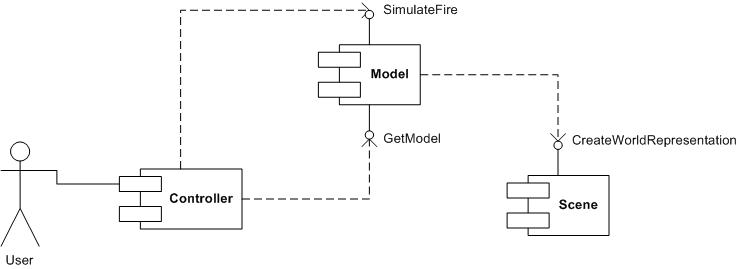
\includegraphics{componentDiagram.jpg} \\
\caption { Architektura aplikacji}
\label {architektura aplikacji}
\end {center}
\end{figure}
Zapewnienie bardzo prostych zależności między modułami pozwala niezależnie rozwijać kolejne części aplikacji, w łatwy
sposób podmieniać i modyfikować ich zachowanie. Inną zaletą zastosowanego modelu jest łatwość
testowania poszczególnych części aplikacji niezależnie.

Przedstawiony model powstał na bazie jednego z najpopularniejszych modeli tworzenia aplikacji wykorzystujących graficzny interfejs użytkownika: Model-View-Controller. Elementem różniącym przedstawiony powyżej model od tradycyjnej architektury Model-View-Controller
jest rozdzielenie elementów GUI pomiędzy dwa moduły:
\begin{itemize}
\item Scene przedstawiającą wyniki aplikacji oraz
\item Controller posiadający zestaw narzędzi dostarczających kontrolę użytkownikowi.
\end {itemize}
Dodatkowo w module Controller zostały połączone elementy widoku wraz z obsługującymi je listenerami.
\subsection{Moduł: Controller}
Moduł kontroler odpowiada za komunikację między użytkownikiem a silnikiem aplikacji. 
Jego podstawowym zadaniem jest dostarczenie łatwego w obsłudze, graficznego interfejsu użytkownika, oraz 
obslugi akcji użytkownika. Wspomniana obsługa akcji może obejmować zarówno zebranie danych ich przetworzenie
i dostarczenie do modelu, pobranie z modelu danych jak i zapis lub kontrolę symulacji.
Funkcjonalności dostarczane przez moduł Controller przedstawia diagram \ref{przypadki uzycia}
\begin{figure}
\begin {center}
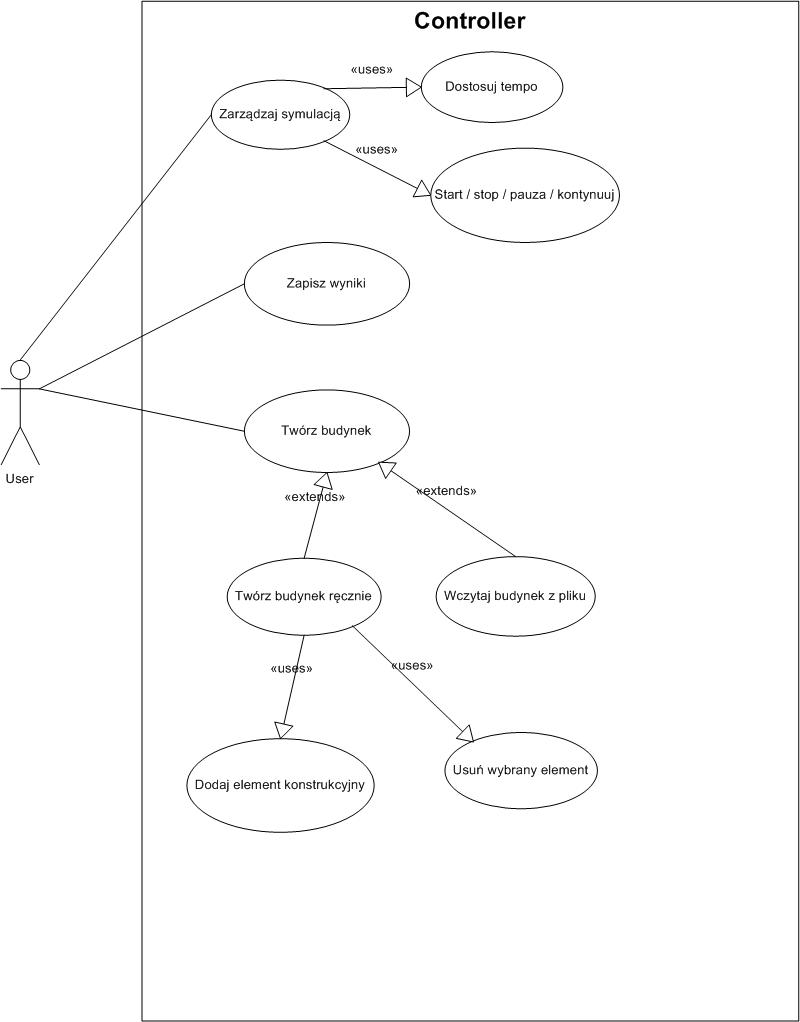
\includegraphics{useCase.jpg} \\
\caption { Przypadki użycia}
\label {przypadki uzycia}
\end {center}
\end{figure}

\subsection {Moduł: Scene}
Jedynym zadaniem sceny jest graficzne przedstawienie dostarczonego modelu.
Całkowite uniezależnienie widoku od innych modułów umożliwia późniejszą jego modyfikację.
\subsection {Model}
Został zastosowany przypadek aktywnego modelu, który potrafi zmieniać swój stan nie tylko w wyniku
akcji użytkownika ale także samoczynnie. Aktywność modelu w przypadku symulacji polega na 
automatycznym uaktualnianiu swojego stanu co pewien, określony okres czasu, a także powiadamianie widoku o 
zachodzących zmianach.

\section {Moduły}
\section {Obiekty}
